\documentclass[a4paper]{article}
\usepackage[top=1in, bottom=1.25in, left=1.25in, right=1.25in]{geometry}
\usepackage{amsmath}
\usepackage{multicol}
\usepackage{graphicx}
\usepackage[utf8]{inputenc}
\usepackage[english]{babel}
\setlength{\parskip}{0.03cm plus4mm minus3mm}
\RequirePackage{ltxcmds}[2010/12/07]
\usepackage{array}
\usepackage{hyperref}
\renewcommand{\arraystretch}{1.5}
%\setlength{\arrayrulewidth}{1mm}
%opening
\title{Homodyne receiver}

\begin{document}

\maketitle

This block of code simulates the reception and demodulation of an optical signal (which is the input signal of the system) outputing a binary signal. A simplified schematic representation of this block is shown in figure \ref{MQAM_receiver_block_diagram_simple}.

\begin{figure}[h]
	\centering
	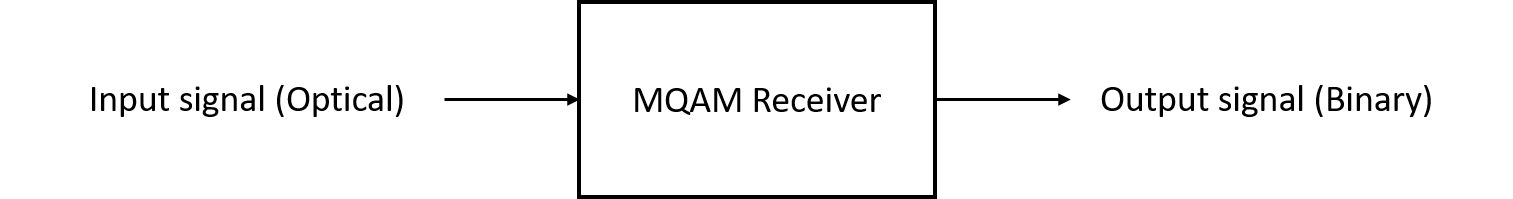
\includegraphics[width=0.8\textwidth]{MQAM_receiver_block_diagram_simple}
	\caption{Basic configuration of the MQAM receiver}\label{MQAM_receiver_block_diagram_simple}
\end{figure}

\subsection*{Functional description}

This block accepts one optical input signal and outputs one binary signal that corresponds to the M-QAM demodulation of the input signal. It is a complex block (as it can be seen from figure \ref{MQAM_receiver_block_diagram}) of code made up of several simpler blocks whose description can be found in the \textit{lib} repository.

In can also be seen from figure \ref{MQAM_receiver_block_diagram} that there's an extra internal (generated inside the homodyne receiver block) input signal generated by the \textit{Clock}. This block is used to provide the sampling frequency to the \textit{Sampler}.


\begin{figure}[h]
	\centering
	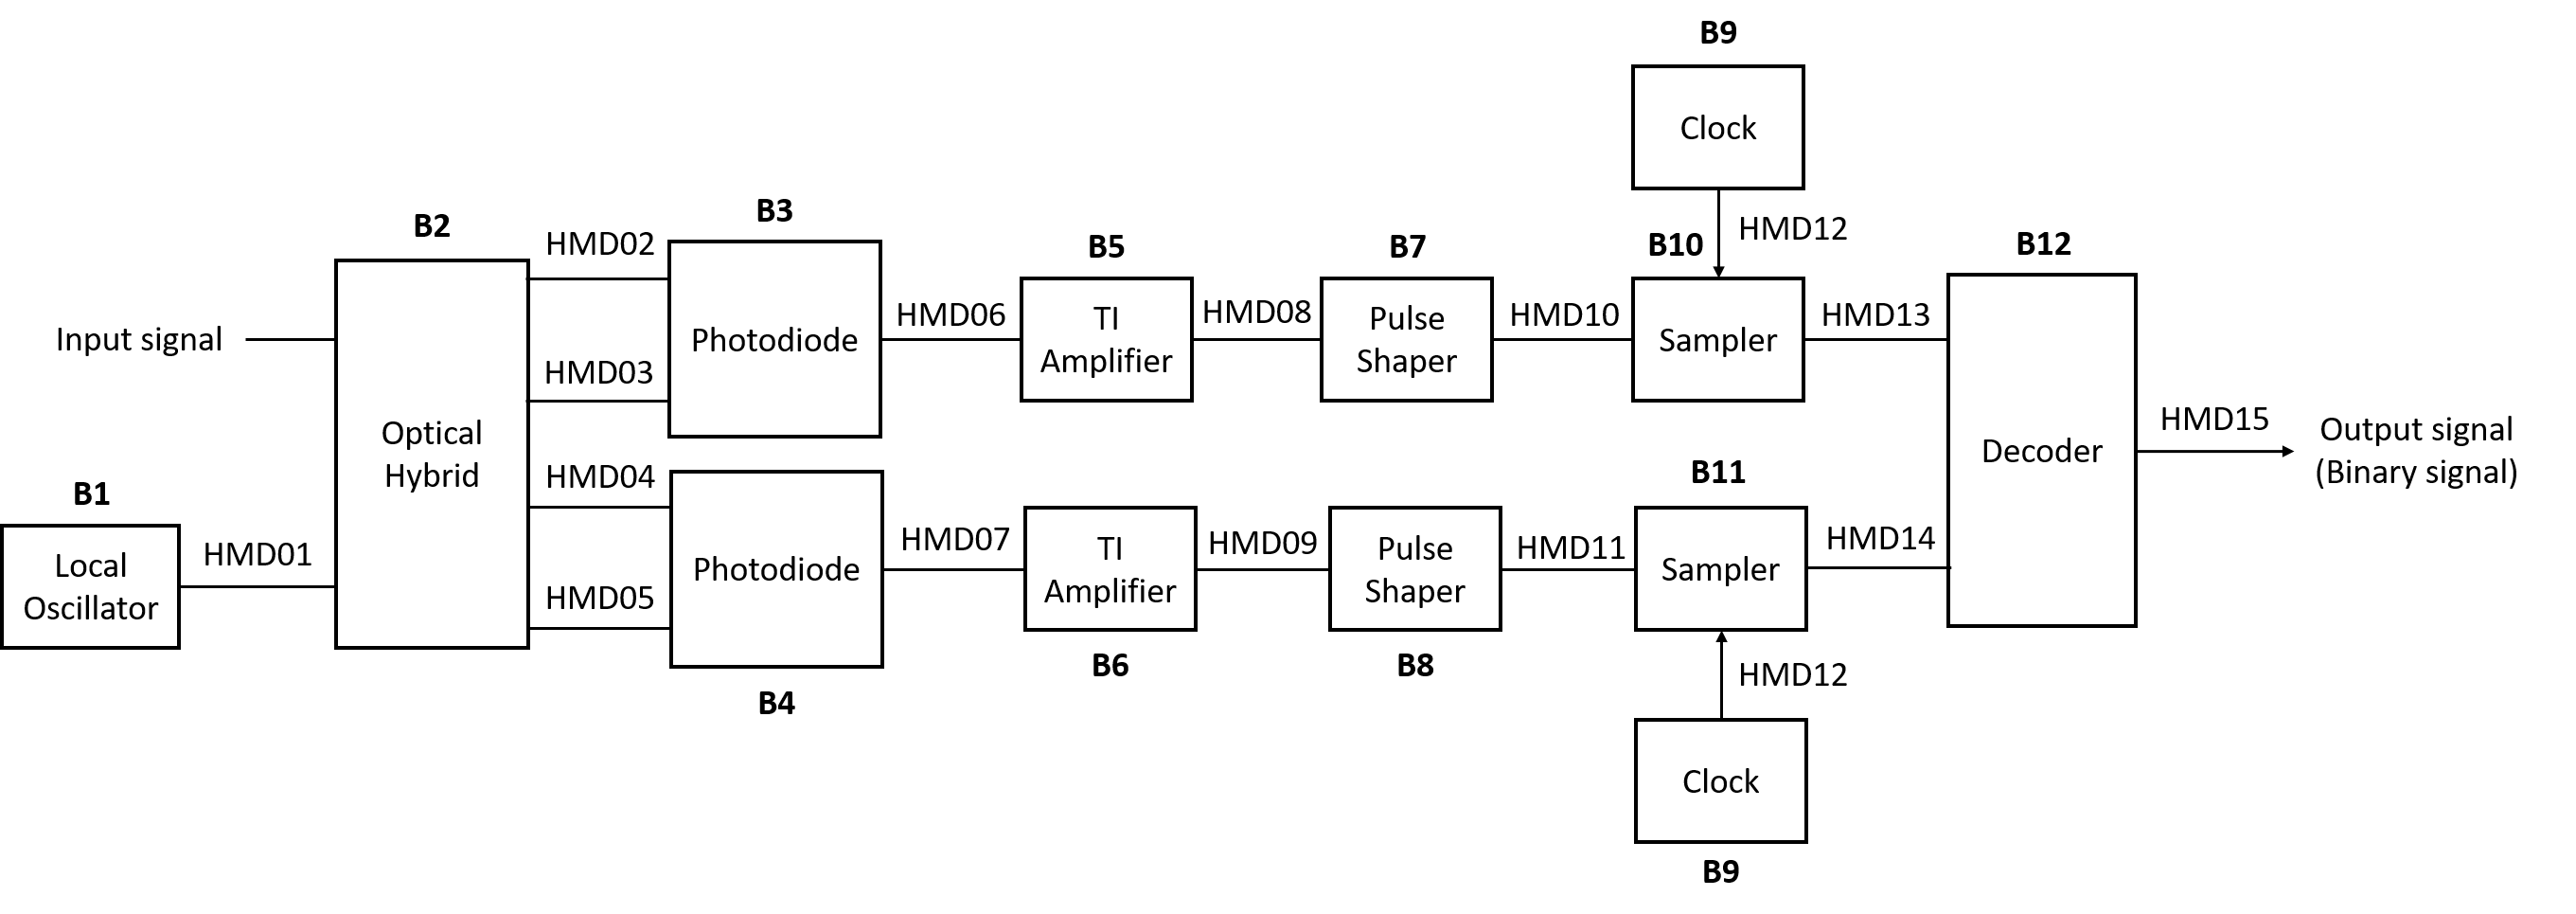
\includegraphics[width=\textwidth]{MQAM_receiver_block_diagram}
	\caption{Schematic representation of the block homodyne receiver.}\label{MQAM_receiver_block_diagram}
\end{figure}

\subsection*{Input parameters}

	\begin{itemize}
		\item samplingPeriod\{0.0\}
		\item localOscillatorOpticalPower\{ 1e-3 \};
		\item localOscillatorPhase\{ 0 \};
		\item localOscillatorWavelength\{ 1550e-9 \};
		\item outputOpticalFrequency{ SPEED\_OF\_LIGHT / localOscillatorWavelength };
	\end{itemize}

\pagebreak

\subsection*{Methods}

HomodyneReceiver(vector$<$Signal *$>$ \&inputSignal, vector$<$Signal *$>$ \&outputSignal) (\textbf{constructor})
\bigbreak
void setIqAmplitudes(vector$<$t\_iqValues$>$ iqAmplitudesValues)
\bigbreak
vector$<$t\_iqValues$>$ const getIqAmplitudes(void) 
\bigbreak
void setLocalOscillatorSamplingPeriod(double sPeriod)
\bigbreak
void setLocalOscillatorOpticalPower(double opticalPower)
\bigbreak
void setLocalOscillatorOpticalPower\_dBm(double opticalPower\_dBm) 
\bigbreak
void setLocalOscillatorPhase(double lOscillatorPhase)
\bigbreak
void setLocalOscillatorOpticalWavelength(double lOscillatorWavelength) 
\bigbreak
void setSamplingPeriod(double sPeriod)
\bigbreak
void  setResponsivity(t\_real Responsivity)
\bigbreak 
void setAmplification(t\_real Amplification) 
\bigbreak
void setNoiseAmplitude(t\_real NoiseAmplitude) 
\bigbreak
void setImpulseResponseTimeLength(int impResponseTimeLength) 
\bigbreak
void setFilterType(PulseShaperFilter fType) 
\bigbreak
void setRollOffFactor(double rOffFactor) 
\bigbreak
void setClockPeriod(double per) 
\bigbreak
void setSamplesToSkip(int sToSkip) 

\pagebreak

\subsection*{Input Signals}

\subparagraph*{Number:} 1 

\subparagraph*{Type:} Optical signal 

\subsection*{Output Signals}

\subparagraph*{Number:} 1 

\subparagraph*{Type:} Binary signal 

\subsection*{Example} 

\subsection*{Sugestions for future improvement}


\end{document}